\documentclass[12pt]{article}

% ----------------------------------------------------------------------
% Define external packages, language, margins, fonts, new commands 
% and colors
% ----------------------------------------------------------------------
\usepackage[utf8]{inputenc} % Codification
\usepackage[english]{babel} % Writing idiom

\usepackage[export]{adjustbox} % Align images
\usepackage{amsmath} % Extra commands for math mode
\usepackage{amssymb} % Mathematical symbols
\usepackage{anysize} % Personalize margins
    \marginsize{2cm}{2cm}{2cm}{2cm} % {left}{right}{above}{below}
\usepackage{appendix} % Appendices
\usepackage{cancel} % Expression cancellation
\usepackage{caption} % Captions
    \captionsetup{labelfont={bf}}
\usepackage{cite} % Citations, like [1 - 3]
\usepackage{color} % Text coloring
\usepackage{fancyhdr} % Head note and footnote
    \pagestyle{fancy}
    \fancyhf{}
    \fancyhead[L]{\footnotesize UMSS} % Left of Head note
    \fancyhead[R]{\footnotesize FCYT} % Right of Head note
    %\fancyfoot[L]{\footnotesize Course} % Left of Footnote
    \fancyfoot[C]{\thepage} % Center of Footnote
    %\fancyfoot[R]{\footnotesize Degree} % Right of Footnote
    \renewcommand{\footrulewidth}{0.4pt} % Footnote rule
\usepackage{float} % Utilization of [H] in figures
\usepackage{graphicx} % Figures in LaTeX
\graphicspath{ {./images/} }
\usepackage[colorlinks = true, plainpages = true, linkcolor = istblue, urlcolor = istblue, citecolor = istblue, anchorcolor = istblue]{hyperref}
\usepackage{indentfirst} % First paragraph
\usepackage[super]{nth} % Superscripts
\usepackage{siunitx} % SI units
\usepackage{subcaption} % Subfigures
\usepackage{titlesec} % Font
    \titleformat{\section}{\Large\bfseries}{\thesection}{1em}{}
    \titleformat{\subsection}{\large\bfseries}{\thesubsection}{1em}{}
    \titleformat{\subsubsection}{\normalsize\bfseries}{\thesubsubsection}{1em}{}
	\fancyfoot[C]{\thepage}

% Random text (not needed)
\usepackage{lipsum}
\usepackage{duckuments}


% Sintax code
\usepackage{xcolor}
\usepackage{listings}
\lstset{
	commentstyle=\color{red},
	keywordstyle=\color{blue},
	numbers=left,
    stepnumber=1,
}


% New and re-newcommands
\newcommand{\sen}{\operatorname{\sen}} % Sine function definition
\newcommand{\HRule}{\rule{\linewidth}{0.5mm}} % Specific rule definition
\renewcommand{\appendixpagename}{\LARGE Appendices}

% Colors
\definecolor{istblue}{RGB}{3, 171, 230}
\definecolor{dkgreen}{rgb}{0,0.6,0}
\definecolor{gray}{rgb}{0.5,0.5,0.5}

%%%%%%%%%%%%%%%%%%%%%%%%%%%%%%%%%%%%%%%%%%%%%%%%%%%%%%%%%%%%%%%%%%%%%%%%
%                                 Document                             %
%%%%%%%%%%%%%%%%%%%%%%%%%%%%%%%%%%%%%%%%%%%%%%%%%%%%%%%%%%%%%%%%%%%%%%%%
\begin{document}

% ----------------------------------------------------------------------
% Cover
% ----------------------------------------------------------------------
\begin{center}
    \begin{figure}
        \vspace{-1.0cm}
        %\includegraphics[scale = 0.3, left]{Images/IST_A.eps} % IST logo
    \end{figure}
    \mbox{}\\[1.0cm]
    \textsc{\Huge CIENCIA DE DATOS}\\[3.0cm]
    \textsc{\LARGE VISUALIZACIÓN}\\[1.0cm]
    \textsc{\LARGE PARA}\\[1.0cm]
    \textsc{\LARGE CIENCIA DE DATOS}\\[3.0cm]
    \HRule\\[0.4cm]
    {\large \bf {PROYECTO DEL MODULO V}}\\[0.2cm]
    \HRule\\[2.0cm]
\end{center}

\begin{flushleft}
    \textbf{Estudiantes:}
\end{flushleft}

\begin{center}
    \begin{minipage}{0.5\textwidth}
        \begin{center}            
            
            \begin{center}
            Herrada Villarroel Andrew Jeremiah\\
            \textit{Ing. Informática}\\
            \href{mailto:jeremiah.herrada.villarroel@gmail.com}{\texttt{jeremiah.herrada.villarroel@gmail.com}}
            \end{center}
            
			\begin{center}
			\end{center}	            
            
            \begin{center}
            Perez Zabalaga Jhosimar\\
            \textit{Ing. Informática}\\
            \href{mailto:ramisohj@gmail}{\texttt{ramisohj@gmail}}
            \end{center}
            
            \begin{center}
			\end{center}
            
        \end{center}
    \end{minipage}%
\end{center}

\begin{center}
    \large \bf 2025, Marzo 14
\end{center}

\thispagestyle{empty}

\setcounter{page}{0}

\newpage

% ----------------------------------------------------------------------
% Contents
% ----------------------------------------------------------------------
\tableofcontents 

\newpage

% ----------------------------------------------------------------------
% Body
% ----------------------------------------------------------------------
\section{Antecedentes}


\begin{center}
  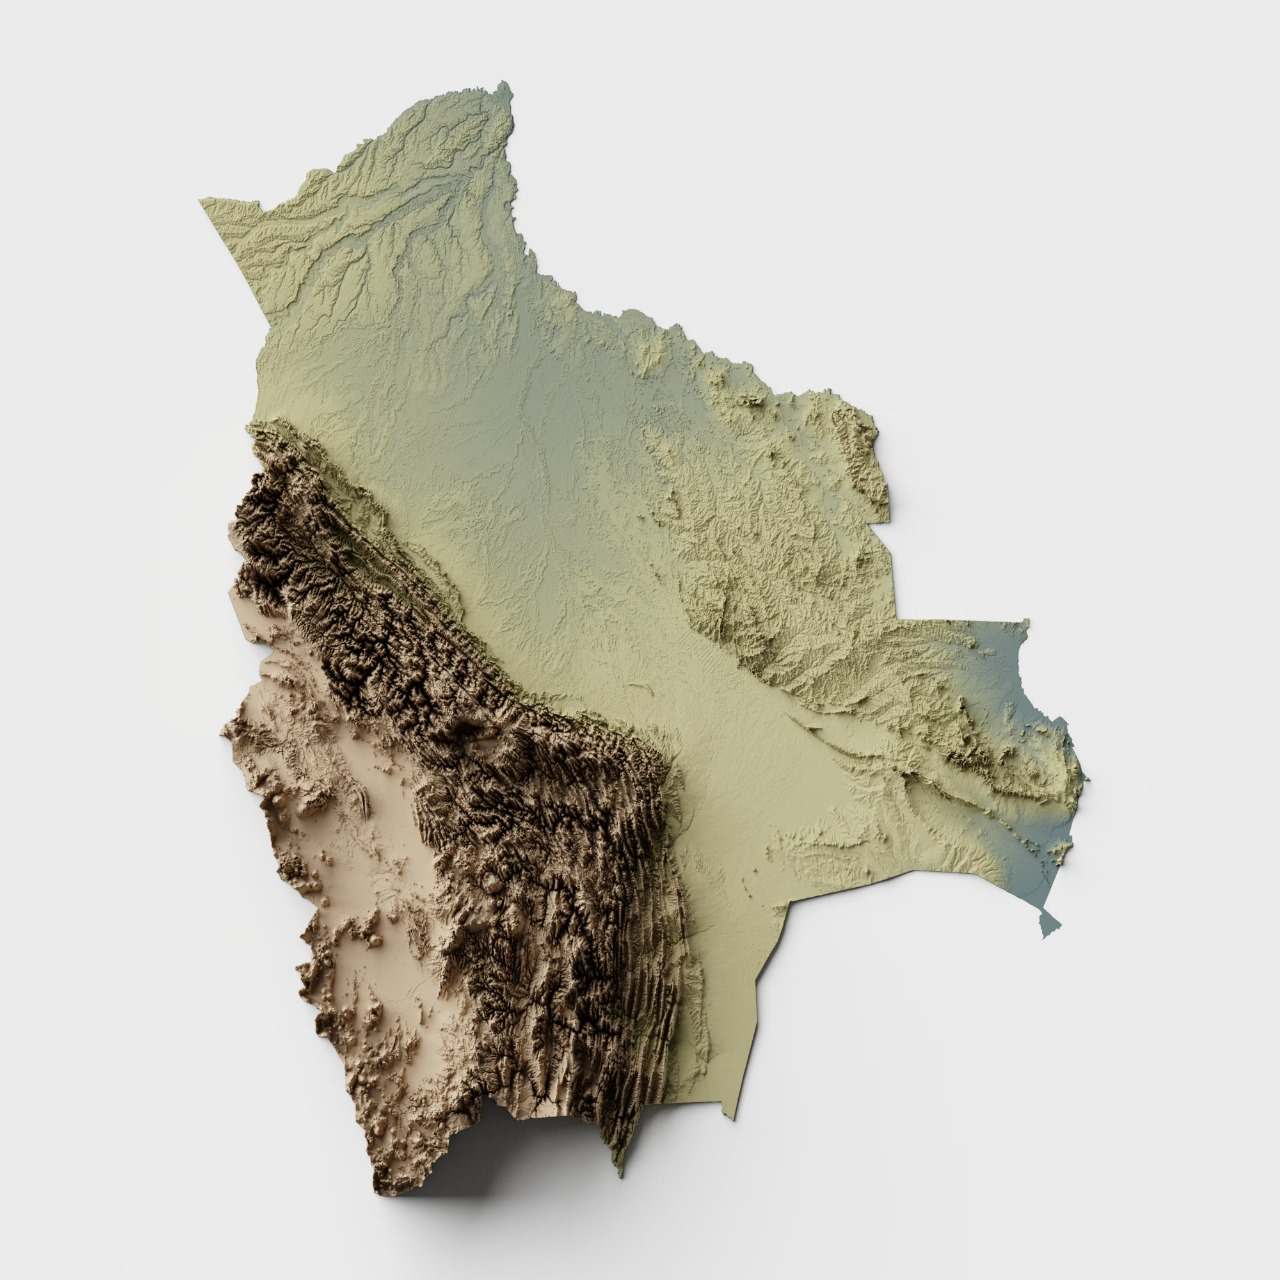
\includegraphics[width=15cm]{bolivian_map}
\end{center}

Bolivia tiene una geografía muy variada, y una de las características principales son sus montañas, los cuales provienen de la cordillera de los Andes que al ingresar al país se divide es dos ramas, cordillera occidental y cordillera oriental, esto fue producido por los diferentes movimientos de las placas tectónicas los cuales son muy recurrentes en el país.
En el cono sur de Cochabamba, a finales de la década de los ’90 se produjo varios terremotos que afectaron gravemente a los municipios de Aiquile, Mizque y Totora. Varias familias quedaron afectadas además que los terremotos en aquella región dejaron grandes pérdidas económicas como también pérdidas humanas.
\\

El siguiente estudio pretende hacer una \textbf{identificación de áreas críticas a partir de datos sísmicos en Bolivia} con respecto a los terremotos. Para tal caso se recopilará datos sísmicos por municipios.


\section{Identificación del problema}

\begin{center}
  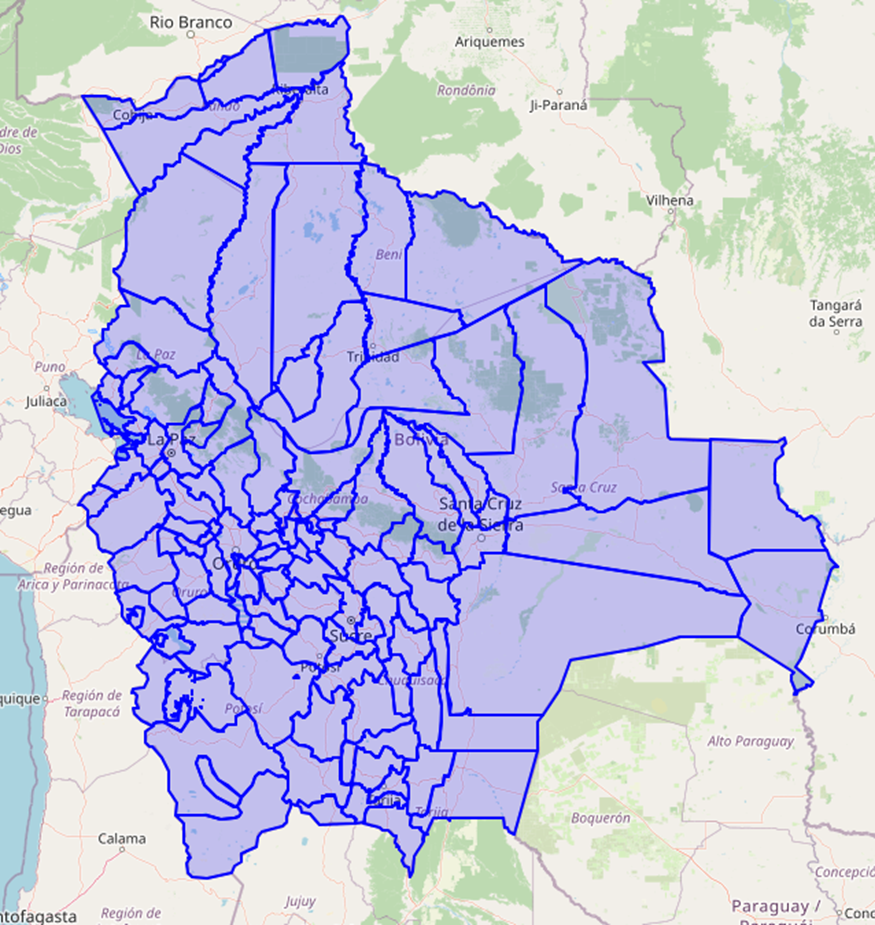
\includegraphics[width=6cm]{bolivia_regiones}
\end{center}

\begin{center}
\textbf{Determinar áreas críticas a partir de datos sísmicos en Bolivia.}
\end{center}

\begin{center}
  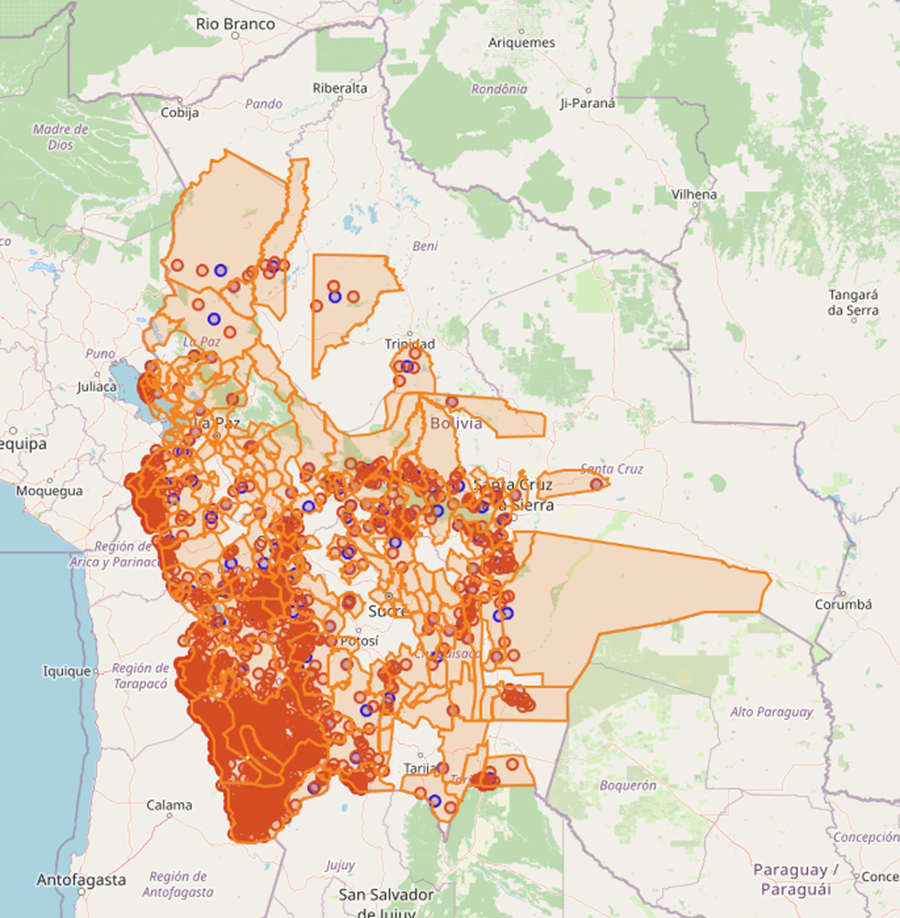
\includegraphics[width=6cm]{bolivia_eq1}
\end{center}

Para realizar el análisis de áreas críticas por movimientos sísmicos se requiere la siguiente información:

\begin{itemize}
\item Registro sísmico. (date, location, magnitude, deep)
\item Mapa geografico de:
	\begin{itemize}
	\item Frontera del país
	\item Departamentos
	\item Provincias
	\item Municipios
	\end{itemize}
\item Mapa geológico de Bolivia.
\item Mapa de asentamientos urbanos.

\end{itemize}




\section{Análisis del problema}

Para realizar el siguiente estudio, es necesario los datos sísmicos, datos geográficos, datos urbanísticos, con los cuales se tiene que trabajar en los siguientes puntos:

\begin{itemize}
\item Identificar patrones y zonas con alta actividad sísmica.
\item Determinar áreas críticas con mayor vulnerabilidad.
\item Facilitación en la toma de decisiones para la gestión de riesgos y la prevención de desastres.
\end{itemize}


\section{Análisis  de los datos}

Para realizar un análisis efectivo, se obtuvieron los siguientes datos:

\begin{itemize}
\item Datos históricos de sismos desde 2009 hasta la fecha actual. \textbf{(3865 records)}
\item Mapas geográficos del país, departamentos, provincias, municipios. \textbf{(GeoJSON files)}
\end{itemize}

\subsection{Datos históricos de sismos}

Los datos sísmicos son proporcionados a través del \textbf{Observatorio San Calixto}, que es una fundación privada, cuya principal actividad es el monitoreo y vigilancia de la actividad sísmica en Bolivia.


\begin{center}
  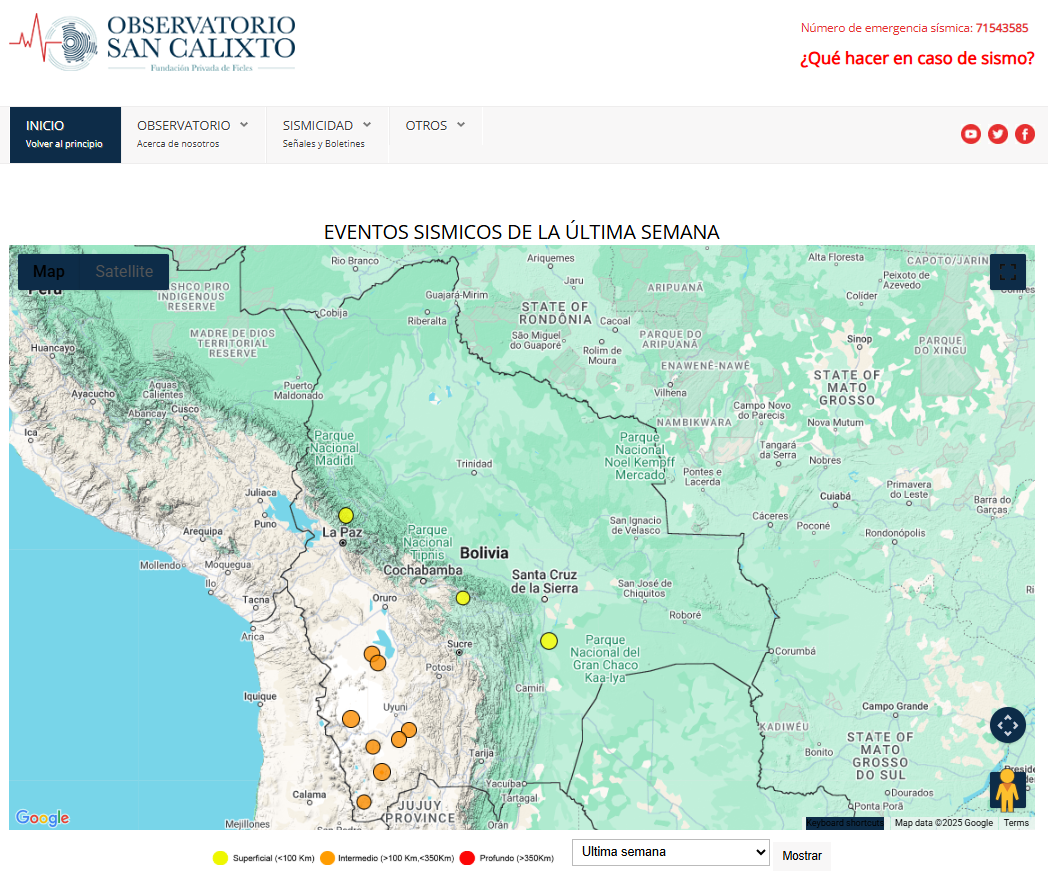
\includegraphics[width=5cm]{san_calixto}
\end{center}


Para obtener todos los datos, se hizo un parser que navegaba a través de cada página por cada uno de los sismos registrados en el sitio oficial del observatorio. Esta etapa se llamó extracción de datos.\\
La siguiente etapa fue la transformación de los datos en información válida, omitiendo los campos nulos, haciendo un tipado de los datos a sus correctivos formatos. La localización de cada sismo  se guardó en formato de geodata. (Point que es representado por coordenadas: longitud, latitud)\\
Por último, se guardó esta información en formato \textbf{GeoJSON} para que pueda ser importada desde cualquier herramienta. En Tableau se importó el archivo como Spatial File.\\

La validación de los registros sísmicos también se hizo mediante \textbf{PostgreSQL}, usando su extensión de \textbf{PostGIS}, con el cual se observó que algunos registros sísmicos pertenecían a otros países, se omitieron \textbf{85} registros.
Los registros sísmicos válidos son \textbf{3865}, los cuales fueron exportados en formato \textbf{GeoJSON} para su posterior tratamiento en \textbf{Tableau}.

\begin{center}
\begin{tabular}{c}
	\hline\hline 
	\textbf{Todos los registros sísmicos}
	\\ 
	\hline 
	\\[-1.5ex]
  	\includegraphics[width=12cm]{out\_bolivia}
  	\\[1ex]
  	\hline\hline
	\textbf{Registros sísmicos válidos}
	\\
	\hline
	\\[-1.5ex]
	 \includegraphics[width=12cm]{in\_bolivia}
	\\[1ex]
	\hline\hline 
\end{tabular}
\end{center}


\subsection{Mapas geográficos}

Los mapas geográficos se obtuvieron mediante archivos \textbf{GeoJSON}, el cual utiliza geodata para generar las áreas del país, departamentos, provincias y municipios.
Estos archivos geojson se obtuvieron de un dataset de la página web data de \textbf{OCHA Services}, el cual contenía cuatro archivos que son los siguientes:

\begin{itemize}
\item \textbf{bol\_adm0} (geodata para el mapa del país.)
\item \textbf{bol\_adm1} (geodata para los mapas de los departamentos.)
\item \textbf{bol\_adm2} (geodata para los mapas de las provincias.)
\item \textbf{bol\_adm3} (geodata para los mapas de los municipios.)
\end{itemize}

\begin{center}
\begin{tabular}{c c}
	\hline\hline 
	\textbf{bol\_adm0} & \textbf{bol\_adm1}
	\\
	\hline & \\[-1.5ex]
  	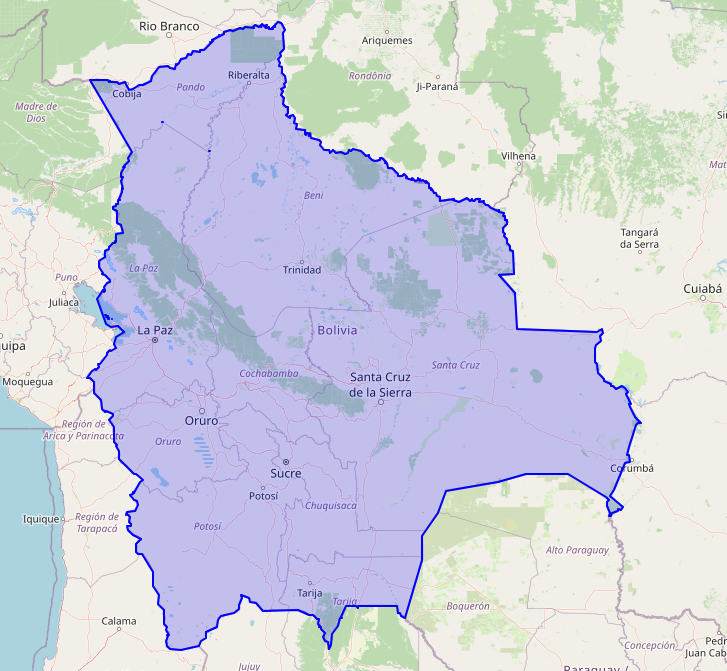
\includegraphics[width=8cm]{adm0}
	&
  	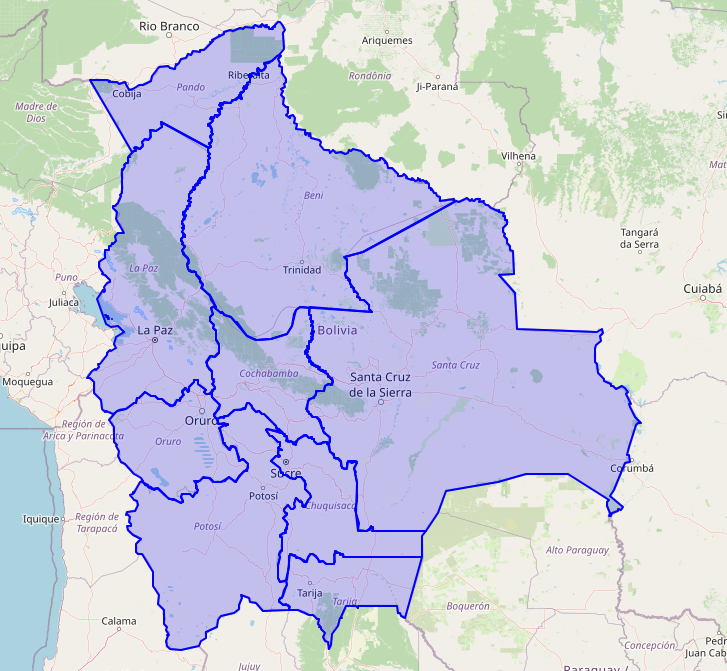
\includegraphics[width=8cm]{adm1}
	\\ [0.5ex]
	\hline\hline
		\textbf{bol\_adm2} & \textbf{bol\_adm3}
	\\
	\hline & \\[-1.5ex]
  	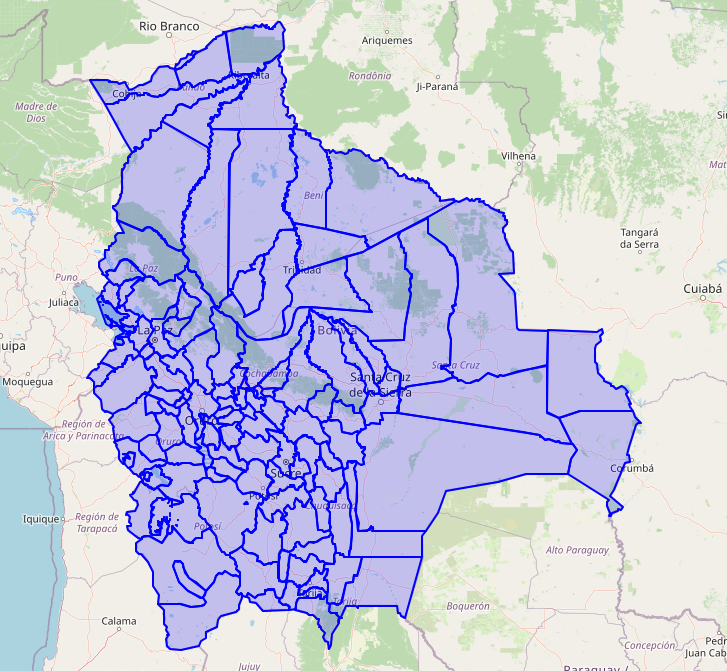
\includegraphics[width=8cm]{adm2}
	&
  	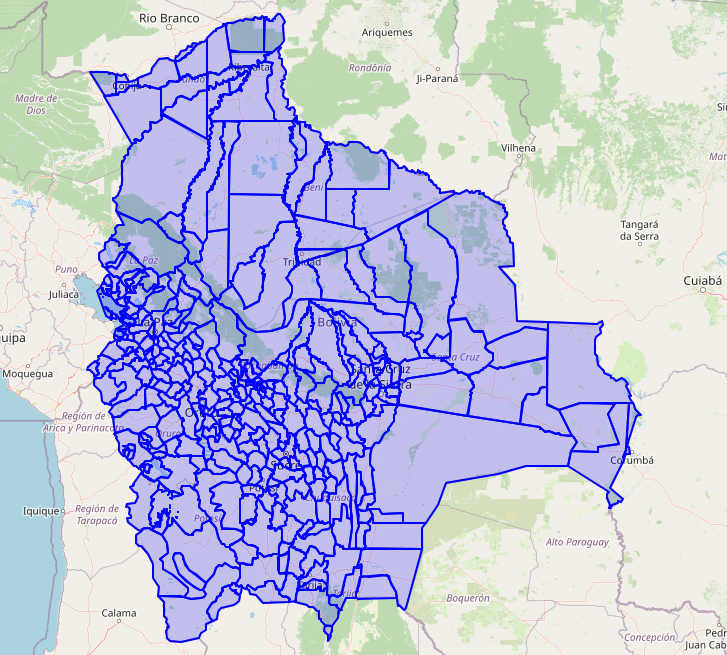
\includegraphics[width=8cm]{adm3}
	\\[1ex]
	\hline\hline & \\[-1.5ex]
\end{tabular}
\end{center}

\section{Resultados de las muestras}

\begin{center}
  \includegraphics[width=17cm]{tableau\_init}
\end{center}

En los resultados del proyecto se pudo clasificar a las regiones en dos grupos, aquellos municipios que tienen actividad sísmica, que mayormente se encuentran en el occidente del país, y los municipios que nos registran actividad sísmica que en su mayoría se encuentran en el oriente.
Existen datos de ciertas regiones donde ya se registran mas de 100 eventos sísmicos contabilizados desde 2009. En total se trabajo con 3865 records para eventos sísmicos los cuales fueron eventos que se suscitaron en 139 municipios de las mas de 340 que existen en el país.






% ----------------------------------------------------------------------
% References
% ----------------------------------------------------------------------

\begin{thebibliography}{00}

\bibitem{b1} Repositorio grupal en Gitlab: big\_data\\
URL: {\url{https://gitlab.com/ramisohj/big_data/-/blob/main/laboratorio_3/docs/laboratorio_3.pdf}}

\bibitem{b1} Repositorio del modelo de identificación de desperdicios: big\_data\\
URL: {\url{https://github.com/AgaMiko/waste-datasets-review}}
\end{thebibliography}


\end{document}